%%%%%%%%%%%%%%%%%%%%%%%%%%%%%%%%%%%%%%%%%
% Beamer Presentation
% LaTeX Template
% Version 1.0 (10/11/12)
%
% This template has been downloaded from:
% http://www.LaTeXTemplates.com
%
% License:
% CC BY-NC-SA 3.0 (http://creativecommons.org/licenses/by-nc-sa/3.0/)
%
%%%%%%%%%%%%%%%%%%%%%%%%%%%%%%%%%%%%%%%%%

%----------------------------------------------------------------------------------------
%	PACKAGES AND THEMES
%----------------------------------------------------------------------------------------

\documentclass{beamer}

\mode<presentation> {

% The Beamer class comes with a number of default slide themes
% which change the colors and layouts of slides. Below this is a list
% of all the themes, uncomment each in turn to see what they look like.

%\usetheme{default}
%\usetheme{AnnArbor}
%\usetheme{Antibes}
%\usetheme{Bergen}
%\usetheme{Berkeley}
%\usetheme{Berlin}
%\usetheme{Boadilla}
%\usetheme{CambridgeUS}
%\usetheme{Copenhagen}
%\usetheme{Darmstadt}
%\usetheme{Dresden}
%\usetheme{Frankfurt}
%\usetheme{Goettingen}
%\usetheme{Hannover}
%\usetheme{Ilmenau}
%\usetheme{JuanLesPins}
%\usetheme{Luebeck}
\usetheme{Madrid}
%\usetheme{Malmoe}
%\usetheme{Marburg}
%\usetheme{Montpellier}
%\usetheme{PaloAlto}
%\usetheme{Pittsburgh}
%\usetheme{Rochester}
%\usetheme{Singapore}
%\usetheme{Szeged}
%\usetheme{Warsaw}

% As well as themes, the Beamer class has a number of color themes
% for any slide theme. Uncomment each of these in turn to see how it
% changes the colors of your current slide theme.

%\usecolortheme{albatross}
%\usecolortheme{beaver}
%\usecolortheme{beetle}
%\usecolortheme{crane}
%\usecolortheme{dolphin}
%\usecolortheme{dove}
%\usecolortheme{fly}
%\usecolortheme{lily}
%\usecolortheme{orchid}
%\usecolortheme{rose}
%\usecolortheme{seagull}
%\usecolortheme{seahorse}
%\usecolortheme{whale}
%\usecolortheme{wolverine}

%\setbeamertemplate{footline} % To remove the footer line in all slides uncomment this line
%\setbeamertemplate{footline}[page number] % To replace the footer line in all slides with a simple slide count uncomment this line

%\setbeamertemplate{navigation symbols}{} % To remove the navigation symbols from the bottom of all slides uncomment this line
}

\usepackage{graphicx} % Allows including images
\usepackage{booktabs} % Allows the use of \toprule, \midrule and \bottomrule in tables

%----------------------------------------------------------------------------------------
%	TITLE PAGE
%----------------------------------------------------------------------------------------

\title[SATToSE 2015]{Collaboration Networks in Software Development: Perspectives from Applying different Granularity Levels using Social Network Analysis - Research in progress} % The short title appears at the bottom of every slide, the full title is only on the title page

\author{Miguel Angel Fernandez, Gregorio Robles and Jesus Gonzalez Barahona} % Your name
\institute[UCLA] % Your institution as it will appear on the bottom of every slide, may be shorthand to save space
{
GSyC/LibreSoft, Rey Juan Carlos University \\ % Your institution for the title page
\medskip
\textit{(ma.fernandezsa@alumnos, grex@)urjc.es; jgb@bitergia.com} % Your email address
}
\date{July 7, 2015} % Date, can be changed to a custom date

\begin{document}

\begin{frame}
\titlepage % Print the title page as the first slide
\end{frame}

%----------------------------------------------------------------------------------------
%	PRESENTATION SLIDES
%----------------------------------------------------------------------------------------

%------------------------------------------------
\section{Additional information} % Sections can be created in order to organize your presentation into discrete blocks, all sections and subsections are automatically printed in the table of contents as an overview of the talk
%------------------------------------------------

\begin{frame}
\frametitle{What is \textit{coopetition}?}
\begin{block}{Coopetition}
% Note: "New hybrid behaviour"
Two or more companies that compete and cooperate with each other at the same time.
\end{block}
\begin{itemize}
\item \textit{Firms competing for the same revenue model (i.e., where rivalry is
expected) tend to collaborate more than firms which do not compete for the same
revenue model}
\item This is related to sociological concept of homophily, which is the tendency of individuals to associate and bond with similar others
\end{itemize}

\end{frame}

%------------------------------------------------
\section{Methodology}
%------------------------------------------------
\begin{frame}
\Huge{\centerline{Methodology}}
\end{frame}
%------------------------------------------------

\subsection{Detailed algorithm}

\begin{frame}
\frametitle{Detailed algorithm I}
\begin{figure}
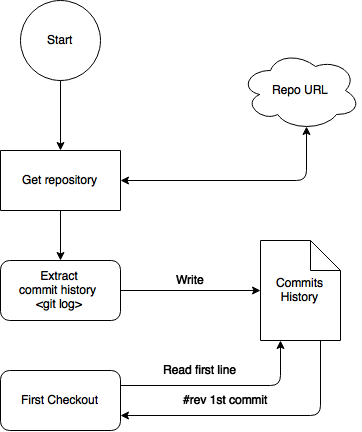
\includegraphics[scale=0.4]{GDCphase1.png} 
\caption{Phase 1 of GraphDataCreator}
\label{fig:phase1}
\end{figure}
\end{frame}

%------------------------------------------------

\begin{frame}
\frametitle{Detailed algorithm II}
\begin{figure}
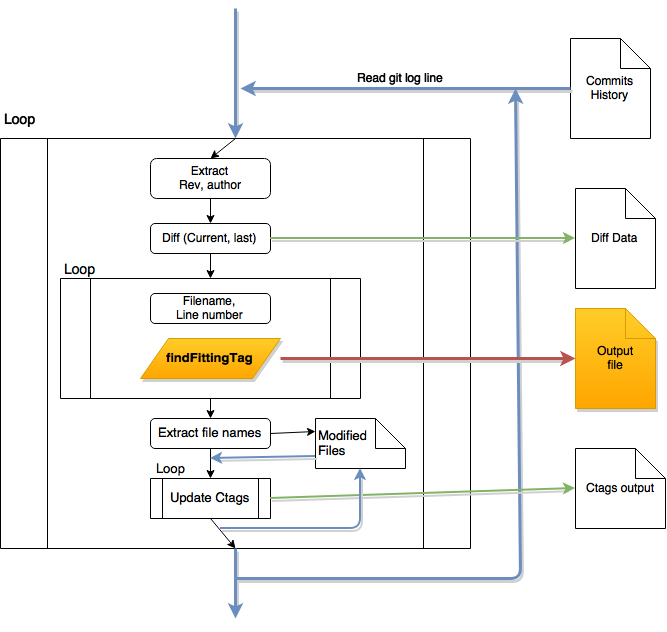
\includegraphics[scale=0.3]{GDCphase2.png} 
\caption{Phase 2 of GraphDataCreator}
\label{fig:phase2}
\end{figure}
\end{frame}

%------------------------------------------------

\begin{frame}
\frametitle{Detailed algorithm: findFittingTag}
\begin{figure}
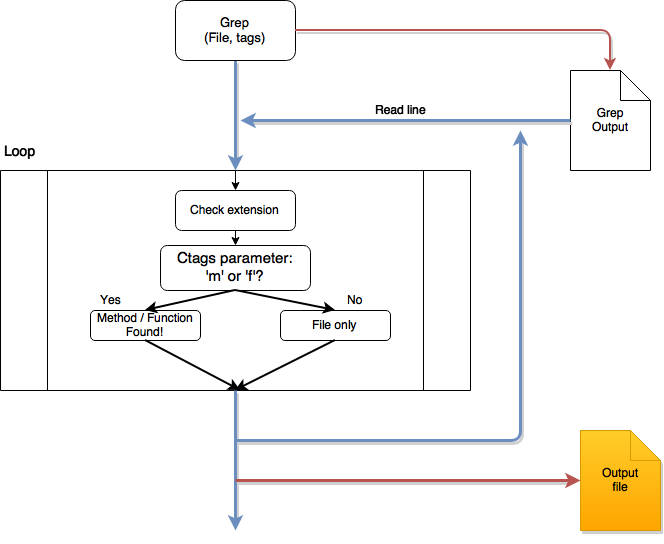
\includegraphics[scale=0.3]{GDCfft.png} 
\caption{Method 'findFittingTag' of GraphDataCreator}
\label{fig:phasefft}
\end{figure}
\end{frame}

%------------------------------------------------

\begin{frame}
\frametitle{Detailed algorithm III}
\begin{figure}
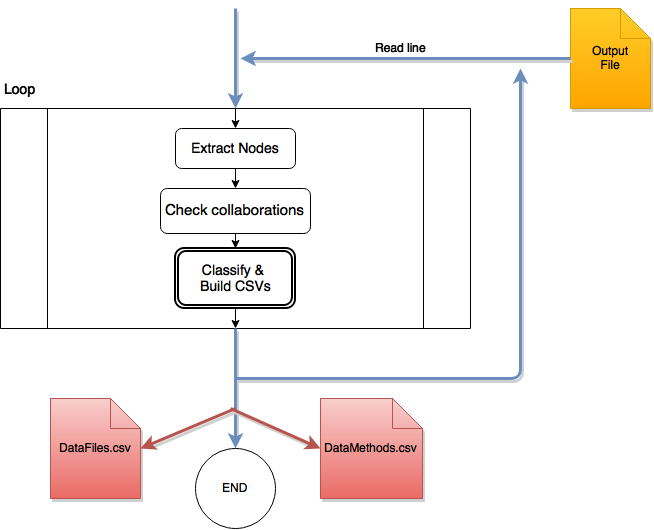
\includegraphics[scale=0.35]{GDCphase3.png} 
\caption{Phase 3 of GraphDataCreator}
\label{fig:phase3}
\end{figure}
\end{frame}

%------------------------------------------------

\begin{frame}
\titlepage % Print the title page as the first slide
\end{frame}

%----------------------------------------------------------------------------------------

\end{document} 